\documentclass[10pt,twocolumn]{article}

\usepackage[a4paper,top=16mm,bottom=17mm,left=16mm,right=16mm]{geometry}
\usepackage[T1]{fontenc}
\usepackage[utf8]{inputenc}
\usepackage{newtxtext,newtxmath}
\usepackage{microtype}
\usepackage{graphicx}
\usepackage{booktabs}
\usepackage{tabularx}
\usepackage{multirow}
\usepackage{amsmath}
\usepackage{xcolor}
\usepackage{enumitem}
\usepackage{caption}
\usepackage{subcaption}
\usepackage{tikz}
\usetikzlibrary{arrows.meta,positioning,shapes.geometric,fit}
\usepackage{hyperref}
\usepackage{fancyhdr}
\usepackage{balance}
\usepackage{needspace}

\definecolor{navy}{HTML}{17324D}
\definecolor{blue}{HTML}{3D6D9A}
\definecolor{teal}{HTML}{2A9D8F}
\definecolor{orange}{HTML}{E88C3A}
\definecolor{pale}{HTML}{EDF3F7}
\definecolor{warning}{HTML}{FFF1C7}

\hypersetup{colorlinks=true,linkcolor=navy,citecolor=blue,urlcolor=blue}
\setlength{\columnsep}{5.5mm}
\setlength{\parindent}{1em}
\setlength{\parskip}{0pt}
\setlist{nosep,leftmargin=*}
\captionsetup{font=small,labelfont=bf}
\pagestyle{fancy}
\fancyhf{}
\fancyhead[L]{MMA Fight Analyzer}
\fancyhead[R]{046217 Deep Learning}
\fancyfoot[C]{\thepage}
\renewcommand{\headrulewidth}{0.3pt}

\newcommand{\projecttitle}{MMA Fight Analyzer: Fight Phase and Pressure Recognition in Broadcast Video}
\newcommand{\macroF}{macro-F1}
\newcommand{\Rtwo}{R(2+1)D}

\begin{document}

\twocolumn[
\begin{center}
  {\LARGE\bfseries\color{navy}\projecttitle\par}
  \vspace{1.5mm}
  {\large Maximilian Bershtman (211754312) \quad Reut Yosefa Vitzner (314743618)\par}
  \vspace{0.7mm}
  {\small Technion -- Israel Institute of Technology, 046217 Deep Learning, Spring 2026\par}
\end{center}
\vspace{1mm}
\begin{minipage}{0.96\textwidth}
\small
\textbf{Abstract.}
We present an end-to-end system that converts UFC broadcast video into an annotated video with a fight/non-fight decision, one of five fight phases, directional pressure, and named fighter boxes every five seconds. We created and labeled 1,315 clips from 11 fights, including 1,159 live-fight clips. The learned pipeline combines a ResNet-18 broadcast-content gate, YOLOv8 person detections, a conservative fighter-identity mask, and Kinetics-pretrained \Rtwo-18 video classifiers. To prevent visual leakage, model selection uses five fight-level development folds and one complete fight remains untouched until all choices are frozen. Development out-of-fold \macroF{} is 0.662 for phase and 0.436 for pressure. On the untouched fight, the gate retains all 156 live clips and rejects 14/19 non-fight clips; phase reaches 72.4\% accuracy and 0.495 \macroF{}, while pressure reaches 35.3\% and 0.327. The results support reliable broad phase recognition, but also expose limited generalization for subjective directional pressure.
\end{minipage}
\vspace{3mm}
]

\section{Introduction}

Understanding an MMA broadcast requires more than recognizing that a fight is present. A useful analysis must distinguish live action from replays and breaks, describe whether the fighters are striking, grappling, clinching, transitioning, or measuring distance, and preserve fighter identity when stating who applies pressure. Automating these decisions can support video indexing, highlight search, coaching review, and explanations for less experienced viewers. The setting is difficult because broadcast cameras move, fighters overlap, referees enter the frame, phases change gradually, and ``pressure'' is intrinsically more subjective than physical position.

This project contributes: (1) a custom, five-second MMA dataset with explicit non-fight examples; (2) an identity-aware four-channel video representation; (3) a leakage-resistant evaluation protocol based on complete fights; (4) systematic comparisons of video backbones, multi-task versus single-task learning, identity masks, head structure, and temporal smoothing; and (5) a Streamlit demonstration that preserves audio and abstains when fighter identity is uncertain.

\subsection{Related work}

Residual networks provide the image backbone used by our gate and LSTM baseline \cite{he2016deep,hochreiter1997lstm}. For video, Tran et al. factorized 3D convolution into separate spatial and temporal operations, defining the \Rtwo{} family and comparing it with R3D and mixed-convolution (MC3) alternatives \cite{tran2018closer}. We use weights pretrained on Kinetics-400, a large human-action dataset \cite{kay2017kinetics}, and fine-tune all layers on MMA clips. In a nearby combat-sport setting, Miyaguchi et al. used a small set of fixed-perspective judo tournament clips to study semi-supervised annotation and classification of match presence, activity, and standing state \cite{miyaguchi2024judo}. Our work instead analyzes moving-camera UFC broadcasts, adds directional pressure and fighter identity, filters non-fight broadcast footage, and returns a complete annotated video. Fighter localization uses the COCO-pretrained Ultralytics YOLOv8n implementation \cite{jocher2023yolov8}; all learned components are implemented in PyTorch \cite{paszke2019pytorch}.

\section{Dataset}

We used a custom Streamlit labeler to divide 11 UFC fights into consecutive, non-overlapping five-second clips. The typical source is 1280$\times$720 at 29.97 fps. For each live-action clip, the annotator selected one phase and one pressure label. Replays, walkouts, round breaks, crowd shots, and other broadcast footage were retained as \emph{excluded} clips to train the gate rather than discarded.

The five phase labels are Striking, Grappling/Ground Work, Clinch, Transition/Takedown, and Neutral/Measuring Distance. Pressure is Fighter 1, Fighter 2, or Mutual. Fighter 1 is defined consistently as the name shown left of the broadcast timer; Fighter 2 is the name on the right. Figure~\ref{fig:data} shows the pronounced imbalance: Striking represents 652/1,159 live clips, whereas Clinch has only 57. Pressure is also imbalanced toward Mutual (567 clips).

Due to time constraints, all phase and pressure labels were assigned by one annotator. Consequently, ambiguous boundaries and especially pressure judgments may reflect one person's interpretation; inter-annotator agreement was not measured. This is both an evaluation limitation and a plausible source of pressure-label noise.

\begin{figure*}[t]
  \centering
  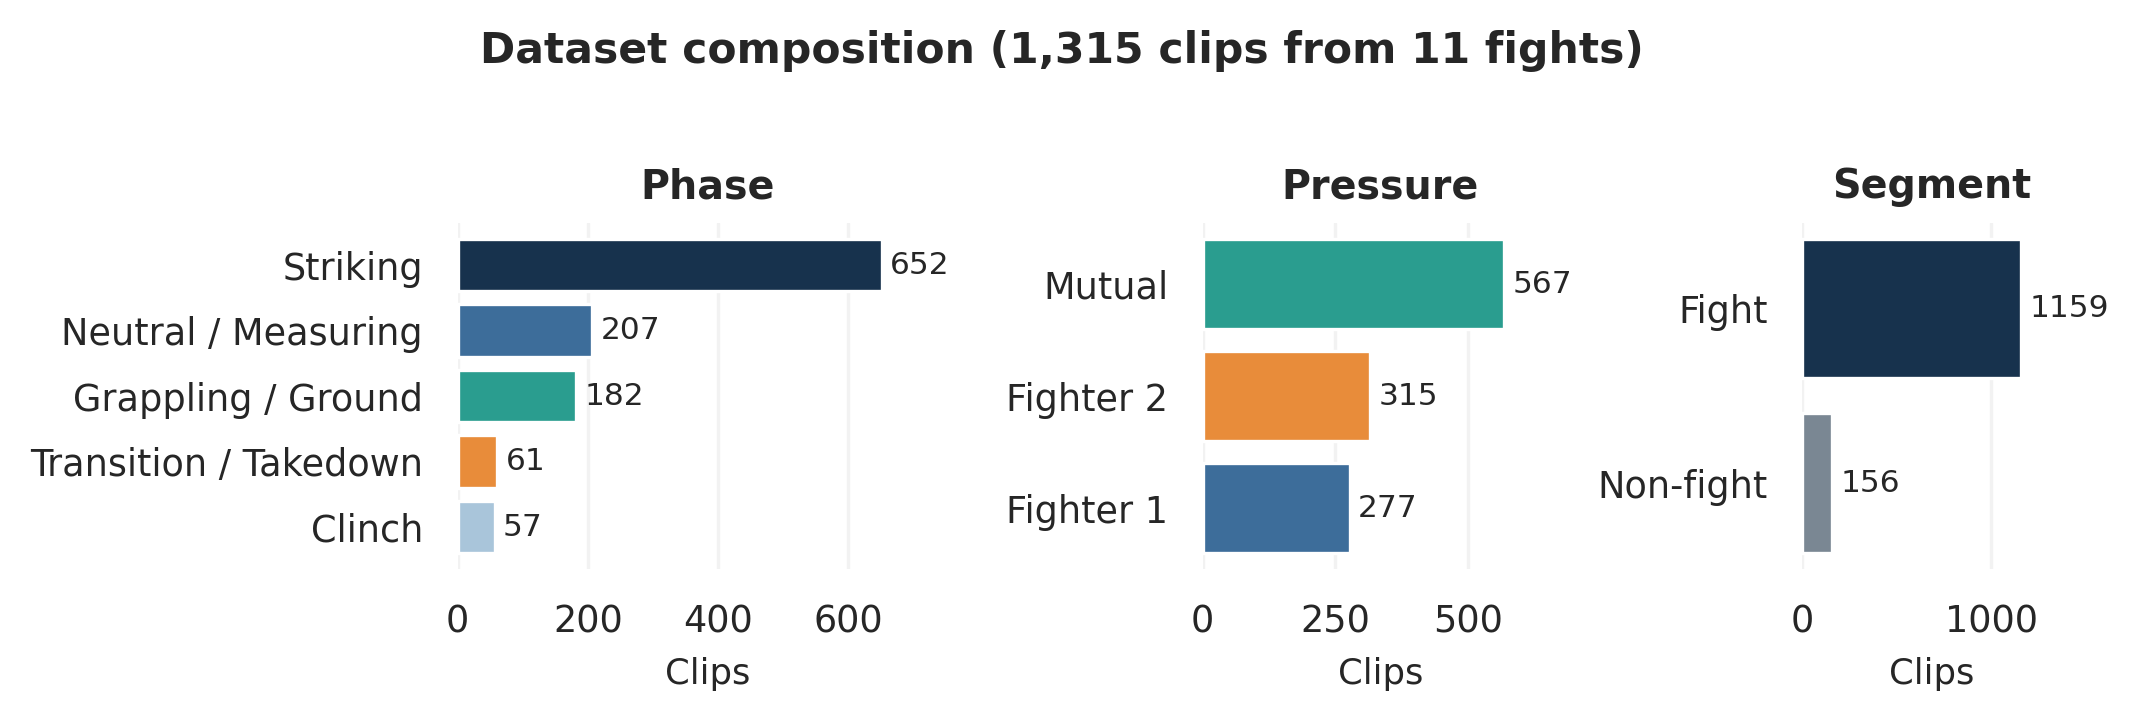
\includegraphics[width=0.98\textwidth]{figures/dataset_distribution.png}
  \caption{Verified dataset composition. The 1,315 clips comprise 1,159 labeled fight clips and 156 non-fight clips.}
  \label{fig:data}
\end{figure*}

\section{Method}

\subsection{Preprocessing and fighter identity}

Each clip is decoded once and sampled at 16 uniformly spaced frames. YOLOv8n runs at the original resolution and retains up to two person detections per frame. Detections are greedily linked across the clip using intersection-over-union (IoU). Training-time identity is assigned at clip level using per-fight shorts-color metadata: the algorithm compares both possible fighter-track pairings using color evidence averaged across the complete tracks. Color ratios are measured over non-skin pixels in the shorts region. Low evidence margins, merged detections, and implausibly small secondary tracks cause abstention rather than a guessed identity.

The assignment is rasterized as a fourth channel: $+1$ inside Fighter 1's box, $-1$ inside Fighter 2's box, and $0$ for background or unknown identity. Overlap is set to zero. The 16 RGB frames are cached at short-side 128 together with the mask; training crops to $112\times112$. This representation makes directional pressure learnable without forcing the network to infer broadcast name order from appearance.

At inference, one A/B prompt associates the two initial tracks with the fighter names. Comparative shorts-color evidence is then fused with temporal appearance and boundary-IoU continuity. Only confident two-track assignments update identity anchors. Merged or low-margin grappling windows abstain, and the overlay reports pressure as uncertain rather than allowing an identity swap.

\subsection{Models}

The \textbf{gate} is an ImageNet-pretrained ResNet-18 with a binary output for non-fight footage. Four cached frames per clip are training examples; at inference their sigmoid probabilities are averaged. The positive-class weight compensates for the 156/1,159 imbalance. A development-only threshold is selected to maximize non-fight rejection while retaining at least 98\% of live-fight clips.

The \textbf{phase/pressure models} receive $x\in\mathbb{R}^{4\times16\times112\times112}$. The primary backbone is Kinetics-pretrained \Rtwo-18 \cite{tran2018closer}. Its first convolution is expanded from three to four channels: pretrained RGB weights are copied, and the mask-channel weights are initialized to zero. The backbone therefore begins with its pretrained RGB behavior. A 512-dimensional clip representation feeds dropout and linear phase/pressure heads. We also evaluate Kinetics-pretrained R3D-18 and MC3-18 under the same protocol. A ResNet-18 plus two-layer LSTM model was implemented during development, but its earlier four-fold results are not mixed with the final five-fold comparison.

The multi-task objective is
\begin{equation}
  \mathcal{L}=\operatorname{CE}_{\mathrm{phase}}+
  0.5\,\operatorname{CE}_{\mathrm{pressure}},
\end{equation}
where each cross-entropy uses training-fold class weights $w_c=N/(K n_c)$ and label smoothing $\epsilon=0.05$. The final phase prediction comes from the selected multi-task model; the final pressure prediction comes from a separately trained pressure-only model because this scored higher on development data.

\begin{figure*}[t]
\centering
\resizebox{\textwidth}{!}{%
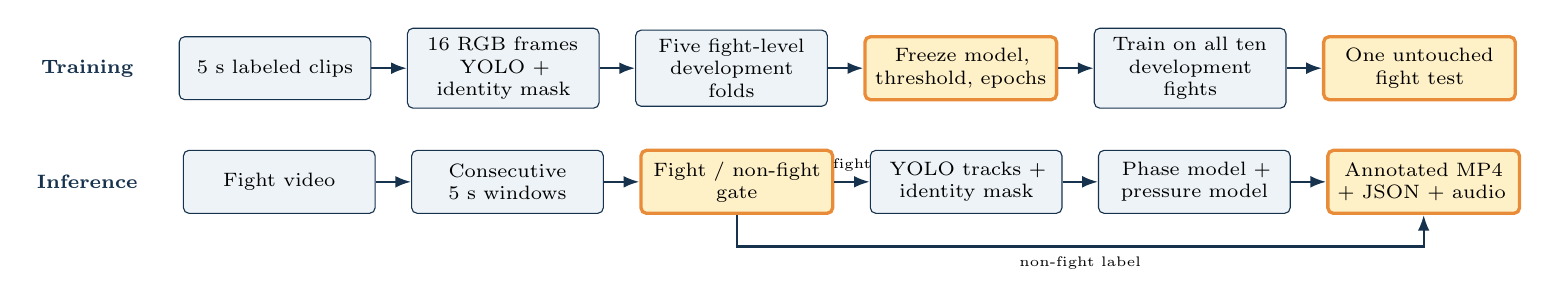
\begin{tikzpicture}[
  stage/.style={draw=navy,rounded corners=2pt,fill=pale,minimum height=8mm,text width=22mm,align=center,font=\scriptsize},
  selected/.style={stage,draw=orange,very thick,fill=warning},
  arrow/.style={-{Latex[length=2mm]},thick,draw=navy},
  note/.style={font=\scriptsize\bfseries,anchor=east,text=navy},
  node distance=3.5mm and 4.5mm
]
\node[note] (trainlabel) {Training};
\node[stage,right=of trainlabel] (clips) {5 s labeled clips};
\node[stage,right=of clips] (prep) {16 RGB frames\\YOLO + identity mask};
\node[stage,right=of prep] (cv) {Five fight-level\\development folds};
\node[selected,right=of cv] (select) {Freeze model,\\threshold, epochs};
\node[stage,right=of select] (final) {Train on all ten\\development fights};
\node[selected,right=of final] (test) {One untouched\\fight test};
\draw[arrow] (clips)--(prep); \draw[arrow] (prep)--(cv); \draw[arrow] (cv)--(select);
\draw[arrow] (select)--(final); \draw[arrow] (final)--(test);

\node[note,below=10mm of trainlabel] (inferlabel) {Inference};
\node[stage,right=of inferlabel] (video) {Fight video};
\node[stage,right=of video] (windows) {Consecutive\\5 s windows};
\node[selected,right=of windows] (gate) {Fight / non-fight\\gate};
\node[stage,right=of gate] (ident) {YOLO tracks +\\identity mask};
\node[stage,right=of ident] (classify) {Phase model +\\pressure model};
\node[selected,right=of classify] (output) {Annotated MP4\\+ JSON + audio};
\draw[arrow] (video)--(windows); \draw[arrow] (windows)--(gate); \draw[arrow] (gate)--node[above,font=\tiny]{fight}(ident);
\draw[arrow] (ident)--(classify); \draw[arrow] (classify)--(output);
\draw[arrow] (gate.south) -- ++(0,-4mm) -| node[pos=0.25,below,font=\tiny]{non-fight label} (output.south);
\end{tikzpicture}
}
\caption{Training and inference workflows. The untouched fight is accessed only after every development choice is frozen.}
\label{fig:pipelines}
\end{figure*}

\subsection{Optimization and augmentation}

All video backbones are fine-tuned with AdamW \cite{loshchilov2019adamw}: the new heads use learning rate $3\times10^{-4}$ and pretrained backbone parameters use $3\times10^{-5}$; weight decay is $10^{-4}$. Training uses mixed precision on CUDA, batch size 8 for \Rtwo/R3D (12 for MC3), a ReduceLROnPlateau scheduler, and early stopping after six unimproved epochs. The monitored development score is phase \macroF{} plus $0.5$ times pressure \macroF{} over the available heads. Random resized crop, horizontal flip, and color jitter are sampled once per clip and applied consistently to all frames; geometric transforms are also applied to the identity mask.

\section{Experimental Protocol}

\subsection{Leakage-resistant splits and metrics}

One complete fight, \emph{Paddy Pimblett vs Michael Chandler}, was fixed as the final holdout before the final experiment suite. Its 156 fight clips and 19 non-fight clips are absent from architecture comparison, early stopping, threshold selection, ablations, hyperparameter trials, and smoothing selection. The other ten fights contain 1,003 live clips and 137 non-fight clips. They form five deterministic validation pairs, so each development fight is validation data exactly once and no clips from a validation fight appear in its training fold.

The primary classification metric is \macroF{}, which weights rare and frequent labels equally; accuracy and per-class precision/recall/F1 are also reported. The gate additionally reports live-fight retention, non-fight rejection, ROC-AUC, and average precision. Out-of-fold (OOF) predictions from all five development folds are concatenated before model selection.

\subsection{Comparisons}

The final protocol evaluates: (i) \Rtwo, R3D, and MC3 multi-task backbones; (ii) multi-task versus phase-only and pressure-only \Rtwo; (iii) pressure with versus without the identity mask; (iv) a flat three-way pressure head versus a hierarchical Mutual/Directional then Fighter-1/Fighter-2 head; (v) learning rate $10^{-4}$ and pressure loss weight 1.0; and (vi) raw predictions versus centered three-window probability averaging and majority vote. Every candidate uses the same five fight pairs. Final epoch counts are the median best epoch from the selected development run: 4 for the gate, 8 for phase, and 10 for pressure.

\section{Results}

\begin{table}[t]
\centering
\caption{Frozen pipeline performance. Gate values are live retention / non-fight rejection; classifier values are accuracy / \macroF{}.}
\label{tab:main}
\small
\begin{tabular}{lcc}
\toprule
Component & Development OOF & Untouched fight \\
\midrule
Gate & 98.0 / 77.4\% & 100.0 / 73.7\% \\
Phase & 72.4 / 0.662 & 72.4 / 0.495 \\
Pressure & 49.8 / 0.436 & 35.3 / 0.327 \\
\bottomrule
\end{tabular}
\end{table}

\subsection{Development selection}

Figure~\ref{fig:models} summarizes the final comparable runs. Multi-task \Rtwo{} achieved the best phase \macroF{} (0.662), narrowly above MC3 (0.656) and above R3D (0.631). Its phase-only counterpart reached 0.636, indicating a 2.7-point benefit from the auxiliary pressure task. For pressure, the separate \Rtwo{} pressure-only model reached 0.436, compared with 0.404 for multi-task \Rtwo, 0.431 for R3D, and 0.421 for MC3.

The identity-mask ablation reduced pressure \macroF{} from 0.436 to 0.423, a modest 1.4-point gain for identity supervision. The hierarchical pressure head scored 0.407. Lowering learning rate to $10^{-4}$ produced 0.650 phase / 0.406 pressure, while increasing pressure weight to 1.0 produced 0.632 / 0.398; neither was selected. Three-window smoothing also hurt both tasks: phase raw/probability/majority \macroF{} was 0.662/0.591/0.640, and pressure was 0.436/0.395/0.403. Therefore deployment uses raw predictions.

\begin{figure*}[t]
  \centering
  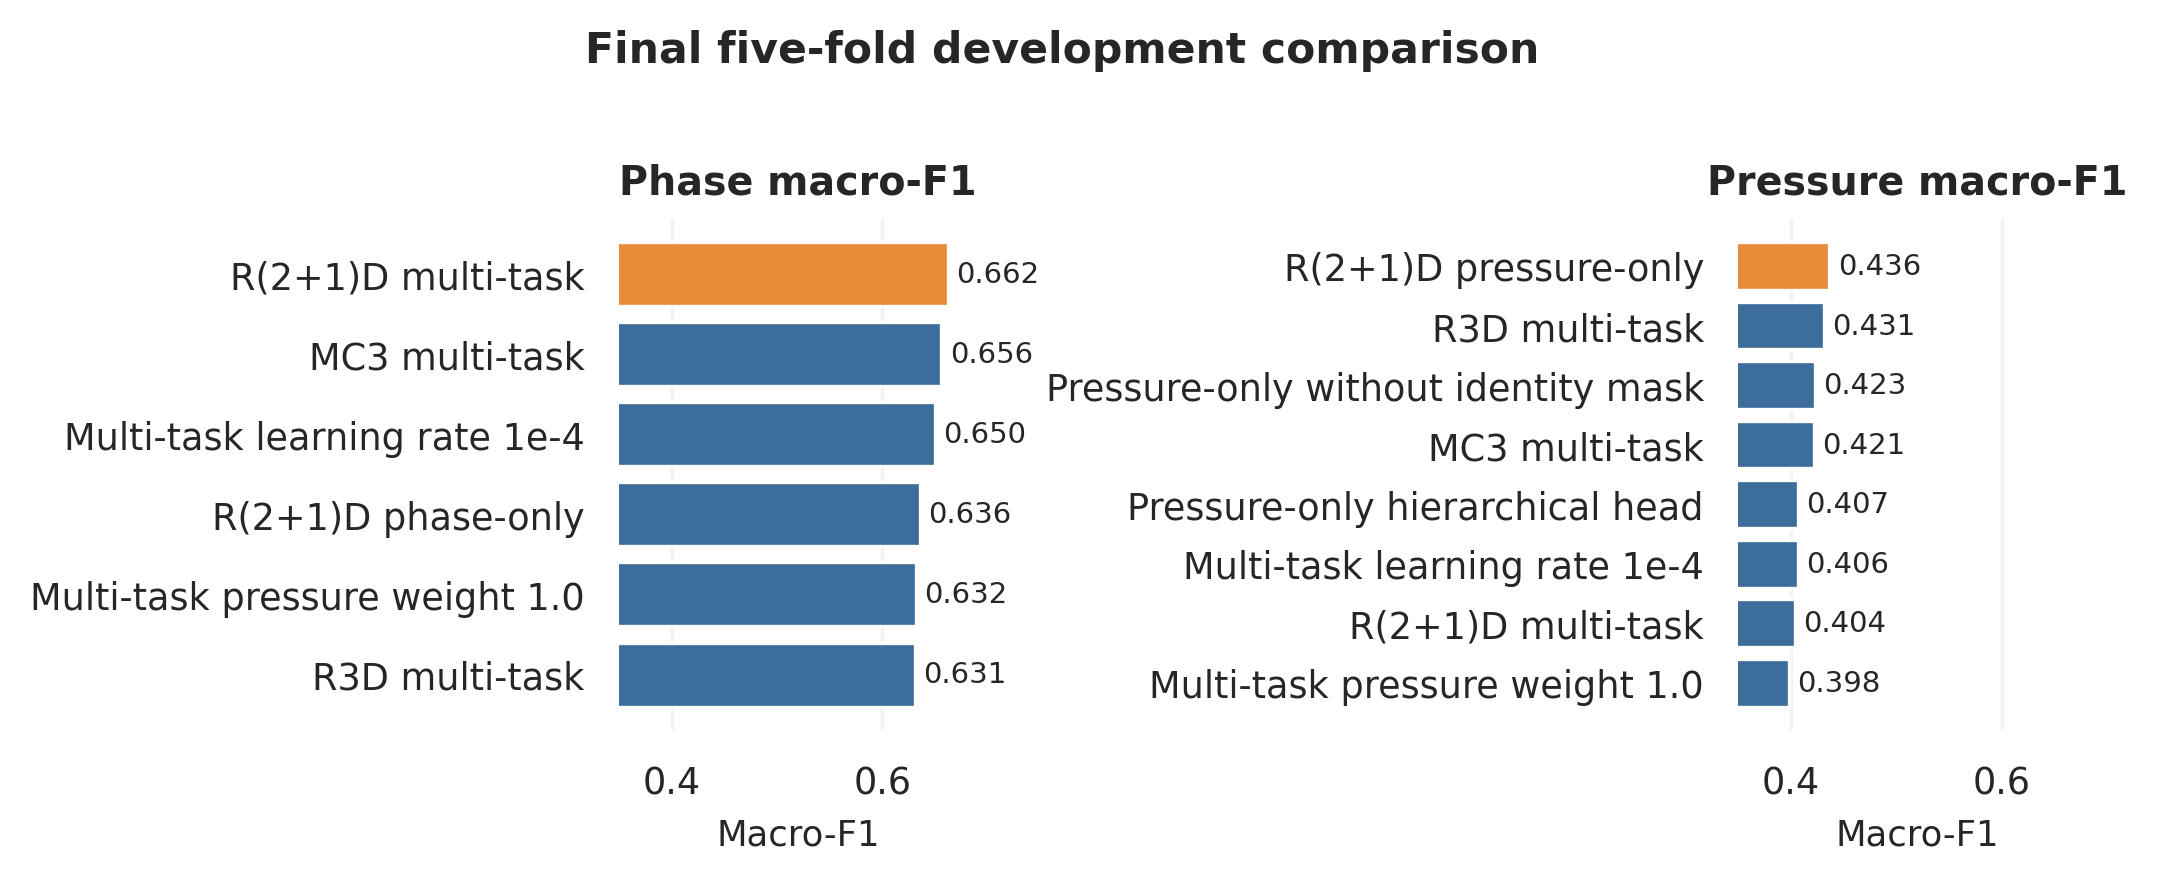
\includegraphics[width=0.98\textwidth]{figures/model_comparison.png}
  \caption{Development OOF comparison. Orange identifies the separately selected phase and pressure models. All bars use the same five fight-level folds.}
  \label{fig:models}
\end{figure*}

\begin{table}[t]
\centering
\caption{Per-class development F1 of the selected models.}
\label{tab:class}
\small
\begin{tabular}{lr@{\qquad}lr}
\toprule
Phase & F1 & Pressure & F1 \\
\midrule
Striking & .809 & Fighter 1 & .287 \\
Grappling/Ground & .791 & Fighter 2 & .387 \\
Clinch & .631 & Mutual & .636 \\
Transition/Takedown & .614 & & \\
Neutral/Measuring & .468 & & \\
\bottomrule
\end{tabular}
\end{table}

\subsection{Untouched-fight evaluation}

The gate retained all 156 real-fight clips and rejected 14 of 19 non-fight clips (ROC-AUC 0.973). Consequently, no downstream fight prediction was lost to the gate. Phase accuracy remained 72.4\%, but \macroF{} fell to 0.495 because the holdout is highly skewed: 79 Grappling clips and only one Clinch clip, which was missed. Striking and Grappling still achieved F1 0.804 and 0.837; Transition and Neutral achieved 0.381 and 0.452.

Pressure showed the central generalization failure: development \macroF{} 0.436 fell to 0.327. Holdout F1 was 0.135 for Fighter 1, 0.341 for Fighter 2, and 0.504 for Mutual. The confusion matrix shows a strong tendency to map directional pressure to Mutual or the wrong fighter. This is consistent with incomplete identity masks, subjective annotation, and a holdout pressure distribution (33/82/41) that differs from development.

\begin{figure*}[t]
  \centering
  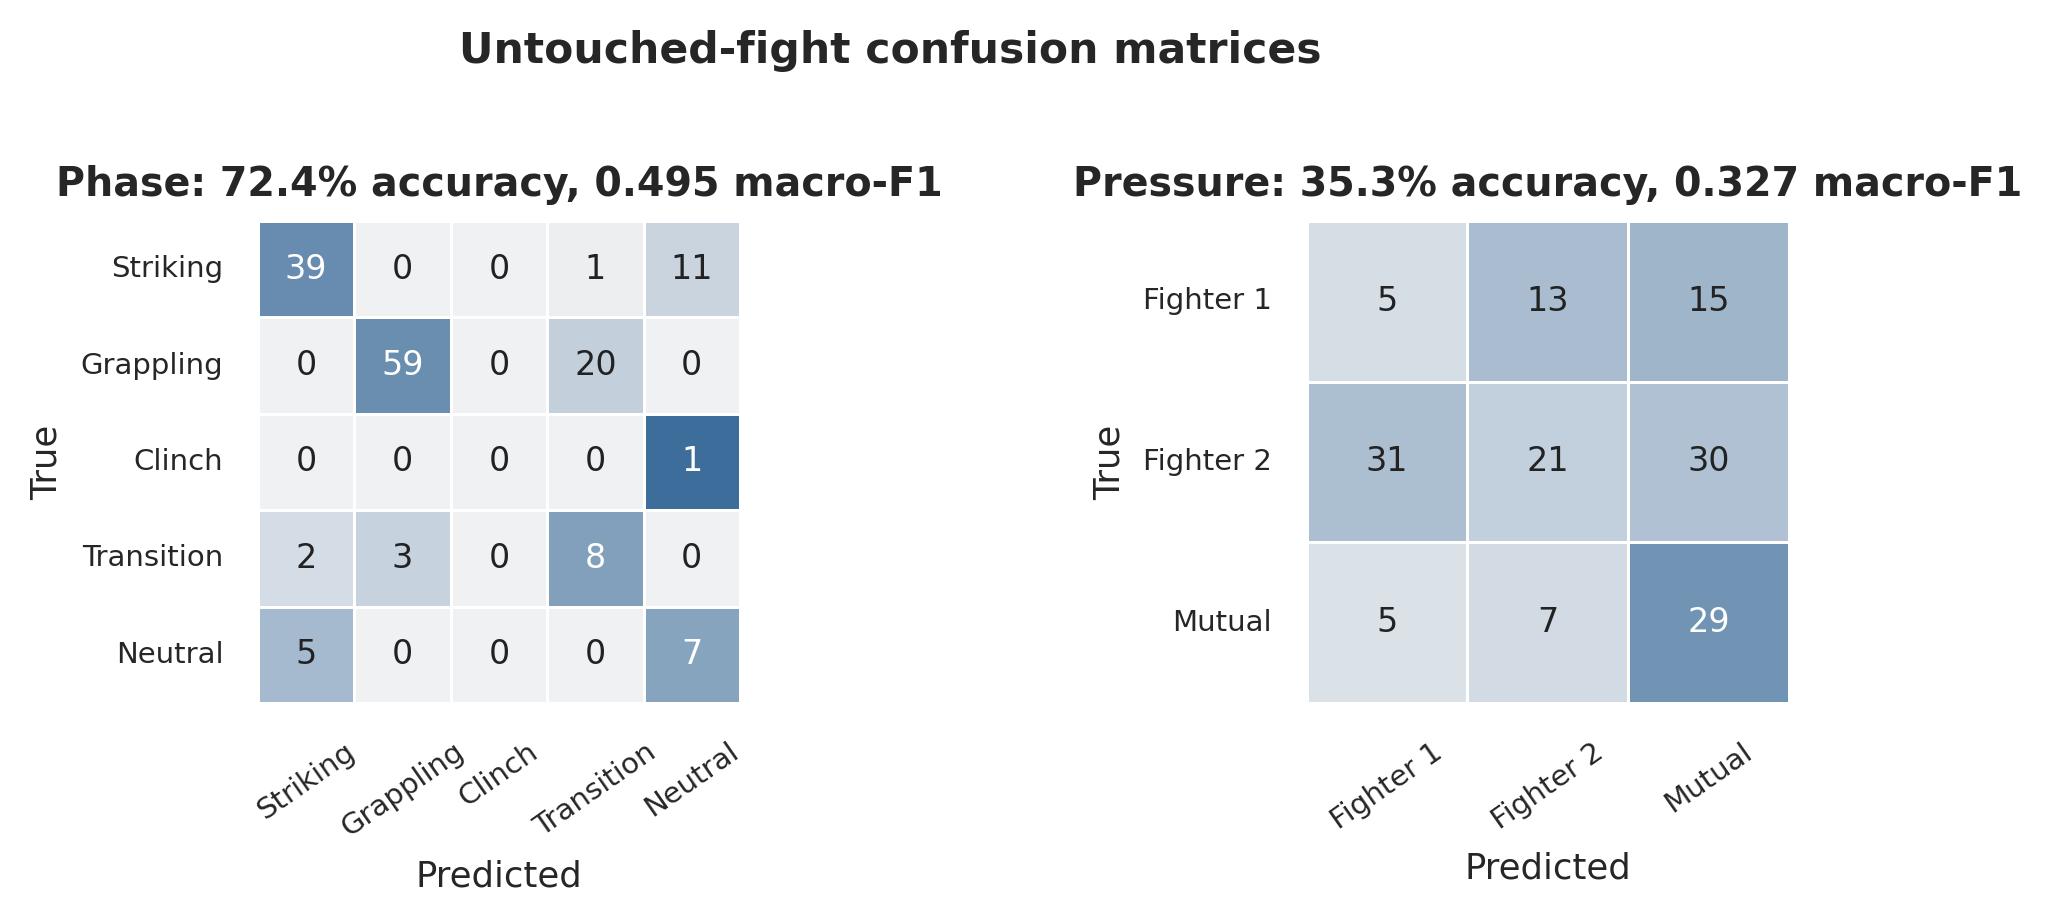
\includegraphics[width=0.98\textwidth]{figures/holdout_confusions.png}
  \caption{Untouched-fight confusion matrices. Cell colors are normalized by true class; annotations are clip counts.}
  \label{fig:confusions}
\end{figure*}

\subsection{End-to-end demonstration}

The Streamlit application executes the same frozen pipeline on the held-out clips or an uploaded video. It asks once which detected box is Fighter 1, displays progress by window, preserves the original audio, and provides the annotated H.264 video and JSON timeline for download. Figure~\ref{fig:demo} shows real outputs. Identity is deliberately withheld when detection or shorts-color evidence is ambiguous.

\begin{figure*}[t]
  \centering
  \begin{subfigure}{0.49\textwidth}
    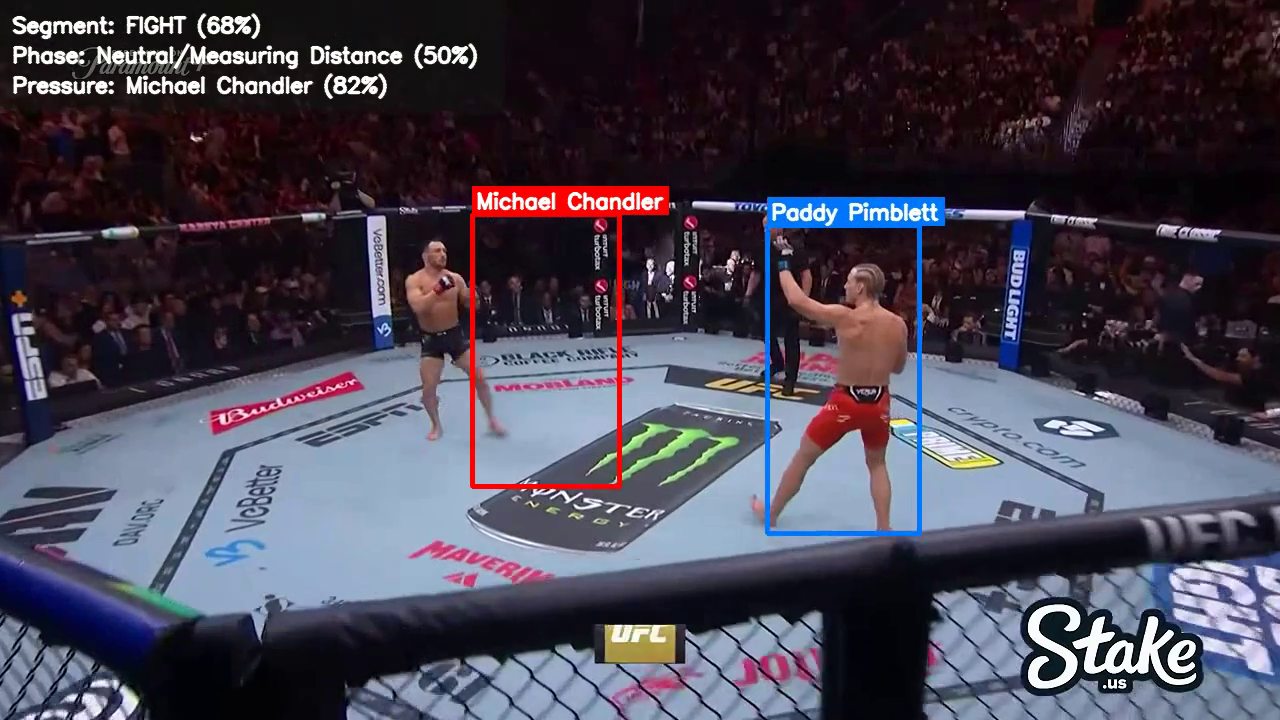
\includegraphics[width=\linewidth]{figures/demo_fight.png}
    \caption{Live window: phase, pressure, confidence, and fighter names.}
  \end{subfigure}\hfill
  \begin{subfigure}{0.49\textwidth}
    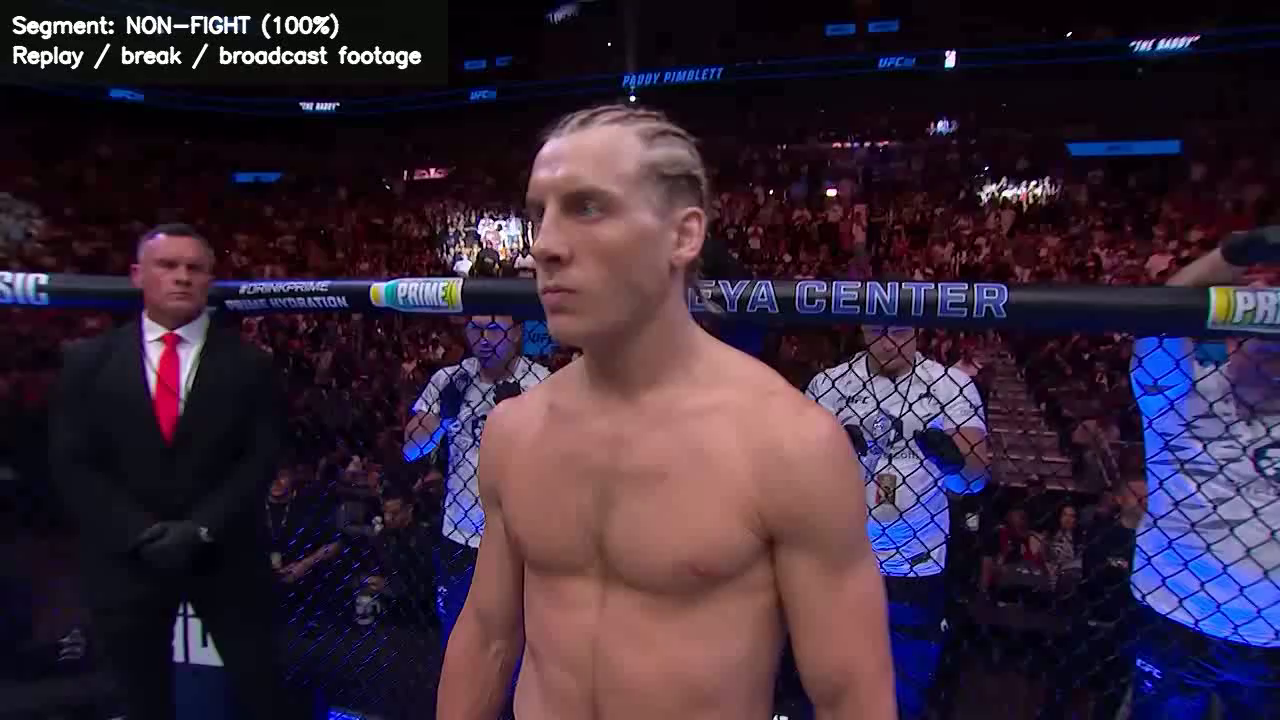
\includegraphics[width=\linewidth]{figures/demo_nonfight.png}
    \caption{Excluded broadcast window routed by the gate.}
  \end{subfigure}
  \caption{Qualitative end-to-end output from the untouched fight.}
  \label{fig:demo}
\end{figure*}

\section{Limitations, Conclusion, and Future Work}

The strongest defensible result is a successful gate-and-phase pipeline. The fixed fight-level protocol prevents the most important source of visual leakage, and the system recognizes Striking and Grappling well. However, 11 fights remain a small domain-specific sample, the single-fight holdout has high variance, and rare classes make \macroF{} unstable. The single annotator introduces unmeasured subjectivity, particularly for pressure. Generic person detection also fails during occlusion: grappling can merge both fighters into one box or promote a referee/crowd region. Abstention prevents some identity inversions but reduces usable pressure information.

Future work should collect more fights and multiple independent labels, report Cohen's $\kappa$ or a similar agreement measure, and define pressure with a stricter annotation rubric. A fighter-specific detector and learned re-identification/tracking model should replace generic YOLO person boxes and fixed color ranges. Longer context or explicit trajectories may help separate Neutral from Striking and stabilize directional pressure. The present system is suitable for academic indexing and explanation, not judging, officiating, betting, or safety-critical decisions.

\clearpage
\onecolumn

\section{Ethics Statement: Project Stakeholders and Implications Assessment}

\noindent\textbf{1. Introduction}

\noindent\textbf{Student names:} Maximilian Bershtman and Reut Yosefa Vitzner.\\
\textbf{Project Title:} \projecttitle.\\
\textbf{Describe your project (2--3 sentences):} The project analyzes MMA broadcast video in five-second windows. It filters non-fight footage, classifies the current fight phase and directional pressure, tracks fighter identities, and produces an annotated video. Its aim is to support transparent video indexing and explanation while exposing confidence and identity uncertainty.

\medskip
\noindent\textbf{2. Have a large language model (LLM) answer the following questions on your project.}\\
\textit{LLM used for Sections 2a--2c: ChatGPT (OpenAI).}

\smallskip
\noindent\textbf{2a. List 3 types of stakeholders that will be affected by the project.}
\begin{enumerate}[label=(\roman*)]
  \item MMA viewers, analysts, and educational-content creators;
  \item fighters, coaches, officials, and promotions whose performances and likenesses appear in the footage;
  \item researchers, developers, and media platforms that may reuse the dataset, code, or predictions.
\end{enumerate}

\noindent\textbf{2b. What will an explanation that is given to each stakeholder look like? (1 paragraph max)}

Viewers and analysts should be told that the labels are model predictions rather than official descriptions, that pressure is substantially less reliable than phase, and that uncertain identity may suppress a pressure name. Fighters, coaches, officials, and promotions should receive the same accuracy limitations together with notice that the model is not validated for scoring, judging, safety, or employment decisions and that broadcast footage and likeness rights remain relevant. Researchers, developers, and platforms should receive the dataset composition, fight-level split, single-annotator limitation, per-class results, failure modes, intended academic use, and sufficient implementation details to reproduce or audit the claims.

\smallskip
\noindent\textbf{2c. Who is responsible for giving the explanation to each stakeholder? (1 paragraph max)}

The project authors are responsible for accurate documentation, model limitations, provenance, and reproducible evaluation in the report and repository. Any organization or developer who deploys or modifies the system becomes responsible for presenting these limitations in the user interface, obtaining the necessary rights and consent for footage, monitoring performance in its own setting, and preventing unsupported high-stakes uses. Responsibility should not be shifted to viewers or fighters who did not design or deploy the system.

\medskip
\Needspace{7\baselineskip}
\noindent\textbf{3. Reflect on the AI output (this section requires your independent, creative thinking. Do not use LLMs for this stage!).}

\smallskip
\noindent\textbf{3a. What do you think needs to be added/changed in the Generative AI responses, to make the explanation more ethical? (1 paragraph max)}

\begin{center}
\fcolorbox{orange}{warning}{\parbox{0.80\textwidth}{\textbf{Required student-authored reflection.} Replace this box with one paragraph written independently by Maximilian and Reut. The course instructions explicitly prohibit using an LLM for Section 3a.}}
\end{center}

\bibliographystyle{ieeetr}
\bibliography{references}

\end{document}
